\documentclass[final,3p,times]{elsarticle}

\usepackage{amsmath,amssymb,amsthm,mathtools}
\usepackage{enumitem}
\usepackage{tikz}
\usetikzlibrary{positioning}

\biboptions{numbers,sort&compress}

\newtheorem{theorem}{Theorem}
\newtheorem{lemma}[theorem]{Lemma}
\newtheorem{proposition}[theorem]{Proposition}
\newtheorem{corollary}[theorem]{Corollary}
\theoremstyle{definition}
\newtheorem{definition}[theorem]{Definition}
\theoremstyle{remark}
\newtheorem{remark}[theorem]{Remark}

\newcommand{\N}{\mathbb{N}}
\newcommand{\Z}{\mathbb{Z}}
\newcommand{\cE}{\mathcal{E}}
\newcommand{\cP}{\mathcal{P}}
\newcommand{\cG}{\mathcal{G}}
\newcommand{\tw}{\mathrm{tw}}
\newcommand{\dist}{\mathrm{dist}}

\begin{document}

\begin{frontmatter}

\title{Constraint-cycle characterizations and a disjunction frontier\\
for asynchronous reachability in freezing automata networks}

\author[inst1]{Alexander Okezue Bell}
\address[inst1]{Department of Mathematics, Stanford University, Stanford, CA, US}

\begin{abstract}
Freezing automata networks are finite-state graph dynamical systems in which each node evolves monotonically with respect to a fixed order on the alphabet.
We study the asynchronous reachability problem under the standard update-or-keep semantics.
We introduce a class of unit-increment freezing networks whose level-dependent enabling conditions are conjunctions of interval constraints on neighbors.
For this class we build a weighted event-constraint digraph and prove that the target configuration is reachable if and only if the digraph contains no positive directed cycle.
This yields a polynomial-time algorithm and constructs an optimal-round schedule.
We then show a sharp disjunction frontier: allowing two-term disjunctive normal forms of width two in enabling conditions makes reachability NP-complete already for Boolean freezing networks with bounded degree.
Finally, we show that reachability is fixed-parameter tractable in the number of disjunctive increment events by branching on disjunct choices and reducing to the conjunctive cycle test.
\end{abstract}

\begin{keyword}
freezing \sep reachability \sep asynchrony \sep constraints \sep parameterization \sep satisfiability \sep complexity
\end{keyword}

\end{frontmatter}

\section{Introduction}

Automata networks are discrete dynamical systems on a finite graph in which each vertex holds a state from a finite alphabet and evolves according to a local rule depending on its neighborhood.
A network is freezing if there is an order on the alphabet such that each vertex evolves monotonically along every orbit.
Freezing dynamics capture diffusion-type processes such as bootstrap percolation and related growth models, and they have been studied extensively from a computational-complexity viewpoint~\cite{goles2024parameterized}.

We study the asynchronous reachability problem for freezing networks under the standard update-or-keep semantics: at each round an arbitrary subset of vertices applies its deterministic update, while all other vertices keep their current state.
The 2024 work of Goles, Montealegre, R{\'\i}os-Wilson and Theyssier establishes a general parameterized-complexity framework for decision problems in freezing dynamics, highlighting parameters such as alphabet size, treewidth and maximum degree~\cite{goles2024parameterized}.
Our aim is complementary: we isolate a natural multi-level freezing subclass for which reachability admits a sharp structural obstruction and a polynomial-time algorithm, and we identify a minimal way to leave that tractable regime.

\subsection{Contributions}

We define conjunctive interval unit-increment freezing networks (CI-UIFNs), in which a node at level $k$ may increment to $k{+}1$ whenever a conjunction of lower and upper bounds on neighbors holds.
For CI-UIFNs we construct a weighted event-constraint digraph $H$ and prove that the target is asynchronously reachable if and only if $H$ has no positive directed cycle (Theorem~\ref{thm:main}).
The minimum number of rounds equals the maximum directed-path weight in $H$ plus one (Proposition~\ref{prop:makespan}).

We show a sharp disjunction frontier: if enabling guards are allowed to be two-term DNFs of width two, then asynchronous reachability becomes NP-complete already for Boolean freezing networks with bounded degree (Theorem~\ref{thm:two-term}).
The frontier is exact: one-term guards (purely conjunctive) give polynomial time, and two terms already give NP-completeness.

We recover tractability by parameterization: in a disjunctive extension of CI-UIFNs, reachability is fixed-parameter tractable in the number of disjunctive increment-events (Theorem~\ref{thm:fpt}).

\section{Preliminaries}

Let $G=(V,E)$ be a finite undirected graph.
For $v\in V$ write $N(v)$ for the neighbor set and $\Delta(G)$ for the maximum degree.
Let $Q$ be a finite alphabet.
A configuration is a map $x\colon V\to Q$.

\begin{definition}[Freezing network]
Let $(Q,\le)$ be a partially ordered alphabet.
An automata network on $G$ with alphabet $Q$ is freezing if along every orbit $(x_t)_{t\ge 0}$ and every $v\in V$ we have $x_t(v)\le x_{t+1}(v)$.
\end{definition}

\begin{definition}[Asynchronous extension]
Let $F\colon Q^V\to Q^V$ be a deterministic automata network with local functions $(F_v)_{v\in V}$.
The asynchronous extension $F^\ast$ is the nondeterministic dynamics where at each round an arbitrary subset $S\subseteq V$ is updated according to $F$ and all other vertices keep their current state.
That is, $y\in F^\ast(x)$ if there exists $S\subseteq V$ such that $y(v)=F_v(x)$ for $v\in S$ and $y(v)=x(v)$ for $v\notin S$.
All guards are evaluated on the previous configuration $x$.
\end{definition}

\begin{definition}[Asynchronous reachability]
Configuration $y$ is asynchronously reachable from $x$ if there exists a finite orbit $x=x_0,x_1,\dots,x_T=y$ with $x_t\in F^\ast(x_{t-1})$ for all $t\ge 1$.
\end{definition}

\section{Conjunctive interval unit-increment freezing networks}

Fix an integer $h\ge 1$ and let $Q=\{0,1,\dots,h\}$ with the usual order.

\begin{definition}[CI-UIFN]\label{def:ciuifn}
A conjunctive interval unit-increment freezing network (CI-UIFN) on $G$ is a deterministic network $F\colon Q^V\to Q^V$ such that for every $v\in V$ and level $k\in\{0,\dots,h-1\}$ there is a guard $\Phi_{v,k}$ which is a conjunction of literals of the form $x(u)\ge a$ or $x(u)\le b$ over neighbors $u\in N(v)$, with $a,b\in Q$, and the local update is
\[
F_v(x)=
\begin{cases}
k+1,&\text{if }x(v)=k<h\text{ and }\Phi_{v,k}(x)\text{ holds},\\
x(v),&\text{otherwise.}
\end{cases}
\]
\end{definition}

The freezing property is immediate.
We fix a CI-UIFN $F$ and study reachability from $x$ to $y$ under $F^\ast$, assuming the necessary condition $x\le y$ throughout.

\subsection*{Events and the event-constraint digraph}

For each $v\in V$ with $y(v)>x(v)$, define the increment-events $e_{v,k}$ for $k=x(v),\dots,y(v)-1$, representing the increment of $v$ from $k$ to $k+1$.
Let $\cE$ be the set of all such events.

We construct a weighted directed graph $H=(\cE,A)$ with edge weights in $\{0,1\}$.
The edges encode precedence constraints that must hold in any reaching orbit.

\medskip
\noindent\textbf{(E1) Chain constraints (weight 1).}
For each $v$ and $k$ with $x(v)\le k<y(v)-1$, add the edge $e_{v,k}\to e_{v,k+1}$ with weight $1$.

\medskip
\noindent\textbf{(E2) Lower-bound guard constraints (weight 1).}
Fix an event $e_{v,k}$ and suppose $\Phi_{v,k}$ contains a literal $x(u)\ge a$.
If $a>y(u)$, then reachability is impossible.
If $a\le x(u)$, no constraint is needed.
If $x(u)<a\le y(u)$, add the edge $e_{u,a-1}\to e_{v,k}$ with weight $1$.
Note that $a\ge 1$ since $a>x(u)\ge 0$.

\medskip
\noindent\textbf{(E3) Upper-bound guard constraints (weight 0).}
Suppose $\Phi_{v,k}$ contains a literal $x(u)\le b$.
If $x(u)>b$, reachability is impossible.
If $y(u)\le b$, no constraint is needed.
If $y(u)\ge b+1$, add the edge $e_{v,k}\to e_{u,b}$ with weight $0$.

\begin{figure}[t]
\centering
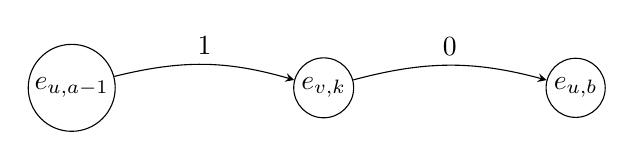
\begin{tikzpicture}[>=stealth, node distance=3.2cm]
\node (A) [circle,draw,inner sep=1.5pt] {$e_{u,a-1}$};
\node (B) [circle,draw,inner sep=1.5pt, right of=A] {$e_{v,k}$};
\node (C) [circle,draw,inner sep=1.5pt, right of=B] {$e_{u,b}$};
\draw[->] (A) to[bend left=15] node[above] {$1$} (B);
\draw[->] (B) to[bend left=15] node[above] {$0$} (C);
\end{tikzpicture}
\caption{Weighted precedence edges from a lower-bound literal $x(u)\ge a$ (weight~$1$) and an upper-bound literal $x(u)\le b$ (weight~$0$).}
\label{fig:edges}
\end{figure}

An edge $a\to b$ of weight $w$ encodes the difference constraint $\tau(b)\ge\tau(a)+w$, where $\tau\colon\cE\to\Z$ assigns an execution round to each event.

\begin{definition}[Positive cycle]
A directed cycle in $H$ is positive if it contains at least one weight-$1$ edge.
\end{definition}

\subsection*{Main characterization}

\begin{theorem}[Reachability iff no positive cycle]\label{thm:main}
Let $F$ be a CI-UIFN on $Q=\{0,\dots,h\}$ with asynchronous extension $F^\ast$.
Given configurations $x\le y$, build the weighted event-constraint digraph $H$, or conclude ``impossible'' if a contradiction arises during construction.
Then $y$ is reachable from $x$ under $F^\ast$ if and only if $H$ contains no positive directed cycle.
\end{theorem}

\begin{proof}
We prove the two implications.

\medskip
\noindent\textit{Only if.}\;
Suppose there is an orbit $x=x_0,x_1,\dots,x_T=y$ under $F^\ast$.
Because updates are unit-increment, each event $e_{v,k}\in\cE$ occurs at a unique round.
Define $\tau(e_{v,k})$ to be the unique $t\in\{1,\dots,T\}$ with $x_{t-1}(v)=k$ and $x_t(v)=k+1$.

We verify that $\tau$ satisfies all constraints $\tau(b)\ge\tau(a)+w$ for each edge $a\to b$ of weight $w$.

For a chain edge $e_{v,k}\to e_{v,k+1}$ of weight~$1$, vertex $v$ cannot increment from both $k$ and $k+1$ in the same round (unit increment), so $\tau(e_{v,k+1})\ge\tau(e_{v,k})+1$.

For a lower-bound edge $e_{u,a-1}\to e_{v,k}$ of weight~$1$, let $t=\tau(e_{v,k})$.
At round $t$ the guard $\Phi_{v,k}$ holds in $x_{t-1}$, giving $x_{t-1}(u)\ge a$.
By orbit monotonicity and unit increment, $u$ reaching level $a$ means $e_{u,a-1}$ occurred by round $t-1$, so $\tau(e_{u,a-1})\le t-1$ and $\tau(e_{v,k})\ge\tau(e_{u,a-1})+1$.

For an upper-bound edge $e_{v,k}\to e_{u,b}$ of weight~$0$, the guard requires $x_{t-1}(u)\le b$.
If $\tau(e_{u,b})<t$ then $u$ would be at least $b+1$ in $x_{t-1}$, a contradiction.
Hence $\tau(e_{u,b})\ge t=\tau(e_{v,k})$.

Since $\tau$ satisfies all constraints, summing around any directed cycle gives $\tau(e)\ge\tau(e)+W$ where $W$ is the total weight.
If $W\ge 1$ this is impossible, so $H$ has no positive cycle.

\medskip
\noindent\textit{If.}\;
Suppose $H$ has no positive cycle.
We construct a valid timing by an iterative Bellman--Ford computation.
Define, for each $n\ge 0$ and event $e$,
\[
\mu_0(e)=0,\qquad
\mu_{n+1}(e)=\max\Bigl(\mu_n(e),\;\max_{(a,e,w)\in A}\mu_n(a)+w\Bigr).
\]
Since $H$ has no positive cycle, every cycle has weight~$0$.
Any walk of length greater than $|\cE|$ contains a repeated vertex, and the subwalk between repetitions is a zero-weight cycle whose removal preserves the walk weight.
It follows by the pigeonhole principle that $\mu_n$ stabilizes at $n=|\cE|$: we have $\mu_n(e)=\mu_{|\cE|}(e)$ for all $n\ge|\cE|$ and all $e$.
Set $\tau(e)=\mu_{|\cE|}(e)+1$.

Then $\tau(e)\ge 1$ for all $e$.
For any edge $(a,b,w)$, the relaxation step gives $\mu_{|\cE|+1}(b)\ge\mu_{|\cE|}(a)+w$, and by stabilization $\mu_{|\cE|+1}(b)=\mu_{|\cE|}(b)$, so $\tau(b)\ge\tau(a)+w$.
Thus $\tau$ is a valid timing.

Let $T=\max_{e\in\cE}\tau(e)$.
For each round $t\in\{1,\dots,T\}$ define
\[
S_t = \{v\in V:\exists k\text{ with }e_{v,k}\in\cE\text{ and }\tau(e_{v,k})=t\}.
\]
Chain constraints give $\tau(e_{v,k+1})\ge\tau(e_{v,k})+1$, so each vertex has at most one event at any round and $S_t$ is well-defined.

Define the orbit $x_0=x$ and $x_t=F^\ast_{S_t}(x_{t-1})$.
We claim, by strong induction on the timing value, that
\begin{equation}\label{eq:invariant}
x_t(v)\ge k+1\quad\text{for all }e_{v,k}\in\cE\text{ with }\tau(e_{v,k})\le t,
\end{equation}
and $x_t(v)\le k$ for all $e_{v,k}\in\cE$ with $\tau(e_{v,k})>t$.

The base case $t=0$ is clear since $x_0=x$ and all events have $\tau\ge 1$.
For the inductive step, consider event $e_{v,k}$ with $\tau(e_{v,k})=t$.
By the chain constraints and the inductive hypothesis at step $t-1$, vertex $v$ has value exactly $k$ in $x_{t-1}$.
We must verify that the guard $\Phi_{v,k}$ holds in $x_{t-1}$.

Consider a literal $x(u)\ge a$ in $\Phi_{v,k}$ with $x(u)<a\le y(u)$.
The edge $e_{u,a-1}\to e_{v,k}$ of weight~$1$ gives $\tau(e_{u,a-1})\le t-1$.
By the inductive hypothesis applied at step $t-1$ (which has strictly smaller timing value for event $e_{u,a-1}$), we get $x_{t-1}(u)\ge a$.

Consider a literal $x(u)\le b$ in $\Phi_{v,k}$ with $y(u)\ge b+1$.
The edge $e_{v,k}\to e_{u,b}$ of weight~$0$ gives $\tau(e_{u,b})\ge t$, so $e_{u,b}$ has not fired by round $t-1$ and $x_{t-1}(u)\le b$.

Literals already satisfied in $x$ or never violated en route to $y$ require no constraint edges and are handled directly.
Thus $\Phi_{v,k}$ holds, and updating $v$ at round $t$ produces the increment $k\to k+1$.

It remains to show $x_T=y$.
The upper bound $x_T(v)\le y(v)$ follows by induction: the orbit never overshoots $y$ because once a vertex reaches $y(v)$, no further needed events exist and guards involving that vertex as an upper-bound target prevent premature increments past $y(v)$.
The lower bound $x_T(v)\ge y(v)$ follows from~\eqref{eq:invariant} applied to the last needed event at $v$.
\end{proof}

\subsection*{Algorithmic consequences}

Theorem~\ref{thm:main} yields a polynomial-time decision procedure.
The graph $H$ has $M=|\cE|\le h|V|$ vertices and $O(M\Delta(G))$ edges.
A positive cycle exists if and only if some weight-$1$ edge has both endpoints in the same strongly connected component.
Thus reachability is decided by one SCC computation plus a scan of all weight-$1$ edges.

\begin{proposition}[Optimal makespan]\label{prop:makespan}
Suppose $y$ is reachable from $x$ and let $L=\max\{W(P):P\text{ is a directed path in }H\}$.
Then every reaching orbit has length at least $L+1$ rounds, and the schedule induced by $\tau$ achieves exactly $L+1$ rounds.
\end{proposition}

\begin{proof}
In any reaching orbit the induced event times satisfy all constraints.
Summing along a path $P$ shows the last event time is at least the first event time plus $W(P)$, so the maximum event time is at least $L+1$.
The timing $\tau$ constructed in Theorem~\ref{thm:main} achieves $\max_e\tau(e)=L+1$.
\end{proof}

\section{A disjunction frontier: NP-completeness for small DNF guards}

We now show that allowing even small disjunctions in enabling conditions makes reachability NP-complete.
Let $Q=\{0,1\}$ with order $0<1$.

\begin{definition}[DNF-guarded freezing Boolean network]
A deterministic Boolean network $F\colon\{0,1\}^V\to\{0,1\}^V$ is DNF-guarded freezing if for each vertex $v$ there is a guard $G_v$ in disjunctive normal form over neighbor literals, and
\[
F_v(x)=
\begin{cases}
1,&\text{if }x(v)=0\text{ and }G_v(x)\text{ is true},\\
x(v),&\text{otherwise.}
\end{cases}
\]
\end{definition}

\begin{lemma}\label{lem:np}
Asynchronous reachability for freezing Boolean networks is in NP.
\end{lemma}

\begin{proof}
Each vertex flips at most once, so any reaching orbit can be compressed to at most $|V|$ effective rounds.
A certificate is a sequence of update sets of length at most $|V|$, verifiable in polynomial time.
\end{proof}

\begin{theorem}[Tovey~\cite{tovey1984simplified}]\label{thm:tovey}
$3$-SAT remains NP-complete when each variable occurs in at most four clauses.
\end{theorem}

\begin{theorem}[NP-completeness with small disjunctions]\label{thm:np}
Asynchronous reachability for DNF-guarded freezing Boolean networks is NP-complete, even when the source is $x\equiv 0$, the target is $y\equiv 1$, every guard is a DNF with at most three terms of width at most two, and the interaction graph has maximum degree at most $6$.
\end{theorem}

\begin{proof}
Membership follows from Lemma~\ref{lem:np}.
We reduce from bounded-occurrence $3$-SAT (Theorem~\ref{thm:tovey}).

Given a $3$-CNF $\varphi$ over variables $X_1,\dots,X_n$ with clauses $C_1,\dots,C_m$, construct a network as follows.
For each variable $X_i$ create two track vertices $t_i,f_i$.
For each clause $C_j$ create a clause vertex $c_j$.
Connect $c_j$ to both $t_i$ and $f_i$ whenever $X_i$ appears in $C_j$.
Each clause vertex has degree~$6$ and each track vertex has degree at most $4$, so $\Delta(G)\le 6$.

Track vertices have the trivially true guard $G_{t_i}\equiv G_{f_i}\equiv\mathrm{true}$.
For a literal $\ell$ on variable $X_i$, define the witness term
\[
T(X_i)=(t_i{=}1)\wedge(f_i{=}0),\qquad
T(\neg X_i)=(f_i{=}1)\wedge(t_i{=}0).
\]
For clause $C_j=(\ell_{j,1}\vee\ell_{j,2}\vee\ell_{j,3})$ set $G_{c_j}=T(\ell_{j,1})\vee T(\ell_{j,2})\vee T(\ell_{j,3})$.

We show $\varphi$ is satisfiable if and only if the all-one configuration is reachable from the all-zero configuration.

Suppose $\alpha$ satisfies $\varphi$.
In round~1, update $t_i$ if $\alpha(X_i)$ is true and $f_i$ if $\alpha(X_i)$ is false.
Track guards are true, so these vertices flip to $1$.
In round~2, update all remaining vertices.
Each remaining track vertex has a true guard and flips to~$1$.
For clause vertex $c_j$, since $\alpha$ satisfies $C_j$ some literal $\ell_{j,r}$ is true.
If $\ell_{j,r}=X_i$ then after round~1 we have $t_i=1,f_i=0$, so $T(X_i)$ holds.
If $\ell_{j,r}=\neg X_i$ then $f_i=1,t_i=0$ and $T(\neg X_i)$ holds.
In either case $G_{c_j}$ is satisfied and $c_j$ flips to~$1$.
After two rounds all vertices are~$1$.

Conversely, suppose there is a reaching orbit.
Define $\alpha(X_i)$ to be true if $t_i$ first reaches~$1$ strictly before $f_i$, and false otherwise.
Fix a clause vertex $c_j$ and let $s$ be the first round at which $c_j$ flips to~$1$.
The guard $G_{c_j}$ holds in the previous configuration, so some witness term $T(\ell_{j,r})$ is true.
If $T(X_i)$ is true then $t_i=1$ and $f_i=0$ at that time, so $t_i$ flipped strictly before $f_i$ and $\alpha(X_i)$ is true, satisfying literal $X_i$.
If both tracks flip simultaneously, neither $T(X_i)$ nor $T(\neg X_i)$ can hold at that time (each requires one track at $0$), so the clause is satisfied by a different literal whose tracks have strict ordering.
Thus $\alpha$ satisfies every clause.
\end{proof}

\begin{remark}
NP-hardness arises from the ability of disjunctions to express alternative witnesses that must be realized in a compatible temporal order.
The conjunctive CI-UIFN regime eliminates this source of nondeterminism and admits the global constraint-graph characterization of Theorem~\ref{thm:main}.
\end{remark}

\section{Fixed-parameter tractability with few disjunctive events}

We extend CI-UIFNs by allowing disjunctions among conjunctive interval terms.

\begin{definition}[Disjunctive interval UIFN]
Fix $h\ge 1$ and $Q=\{0,\dots,h\}$.
A disjunctive interval unit-increment freezing network is a unit-increment freezing network in which each event $(v,k)\colon k\to k{+}1$ has an enabling guard $G_{v,k}=\bigvee_{p=1}^{r_{v,k}}\Gamma_{v,k}^{(p)}$, where each $\Gamma_{v,k}^{(p)}$ is a conjunctive interval guard.
\end{definition}

Fix configurations $x\le y$ and let $\cE$ be the needed increment-events.
Define $K=|\{e_{v,k}\in\cE:r_{v,k}\ge 2\}|$ and $R=\max_{e\in\cE}r_e$.

\begin{theorem}[FPT in the number of disjunctive events]\label{thm:fpt}
Asynchronous reachability for disjunctive interval UIFNs is fixed-parameter tractable parameterized by $K$ and $R$, with running time $O(R^K\cdot\mathrm{poly}(|V|,h,|E|))$.
\end{theorem}

\begin{proof}
For each disjunctive event $e\in\cE$ choose a disjunct index $\sigma(e)\in\{1,\dots,r_e\}$.
There are at most $R^K$ such global choices.
For a fixed $\sigma$, define the CI-UIFN $F^\sigma$ by replacing each guard $G_{v,k}$ with the single conjunct $\Gamma_{v,k}^{(\sigma(e_{v,k}))}$.
Reachability under $(F^\sigma)^\ast$ is decidable in polynomial time by Theorem~\ref{thm:main}.

For soundness, if $y$ is reachable under $(F^\sigma)^\ast$, we construct a reaching orbit for $F^\ast$ using a modified schedule.
The orbit from $(F^\sigma)^\ast$ is retained, but the schedule is filtered to include only vertices where the conjunctive local update $F^\sigma_v$ actually fires.
At any such vertex, the chosen conjunct holds, hence the original disjunction holds, and the disjunctive network $F$ also fires.
At vertices excluded from the filtered schedule, the orbit did not change the vertex value, so no update is needed.
Thus the same orbit witnesses reachability under $F^\ast$.

For completeness, fix a reaching orbit under $F^\ast$.
Each increment event $e_{v,k}$ fires at a unique round (by unit increment and orbit monotonicity).
At that round, some disjunct $\Gamma_{v,k}^{(p)}$ is satisfied.
Choose $\sigma(e_{v,k})$ to be such an index.
The same orbit, with a modified schedule that includes only vertices where $F^\sigma_v$ fires, witnesses reachability under $(F^\sigma)^\ast$.

Therefore $y$ is reachable under $F^\ast$ if and only if it is reachable under $(F^\sigma)^\ast$ for some $\sigma$.
\end{proof}

\section{Further results and applications}

We collect several consequences and extensions of the main results.

\subsection*{SCC characterization}

The positive-cycle test in Theorem~\ref{thm:main} can be reformulated in terms of strongly connected components.

\begin{proposition}\label{prop:scc}
A weighted digraph $H$ with weights in $\{0,1\}$ has a positive directed cycle if and only if some weight-$1$ edge has both endpoints in the same strongly connected component of $H$.
\end{proposition}

\begin{proof}
If $H$ has a positive cycle, it contains a weight-$1$ edge $e=(a,b,1)$.
Since $e$ lies on a cycle from $a$ to $a$, the edge is contained in an SCC.
Splitting the cycle at $e$ gives paths from $b$ to $a$ and from $a$ to $b$ (the edge itself), so $a$ and $b$ are in the same SCC.

Conversely, if a weight-$1$ edge $e=(a,b,1)$ lies within an SCC, there is a path from $b$ back to $a$.
Prepending $e$ yields a cycle through $a$ containing a weight-$1$ edge.
\end{proof}

This gives the decision algorithm stated after Theorem~\ref{thm:main}: compute the SCCs of $H$ in linear time and check whether any weight-$1$ edge is internal to an SCC.

\subsection*{Bootstrap percolation as a special case}

The classical $r$-neighbor bootstrap percolation model on a graph $G$ is the freezing Boolean network where vertex $v$ flips from $0$ to $1$ whenever at least $r(v)$ of its neighbors are $1$.
This is a CI-UIFN with $h=1$ and guard $\Phi_{v,0}$ equal to the conjunction of $r(v)$ literals of the form $x(u)\ge 1$ over $r(v)$ designated neighbors.
Thus Theorem~\ref{thm:main} applies, and we obtain the following.

\begin{corollary}\label{cor:bootstrap}
Asynchronous reachability for $r$-neighbor bootstrap percolation is decidable in polynomial time by the positive-cycle test on the event-constraint digraph.
\end{corollary}

\subsection*{2-CNF interval guards}

A natural intermediate class arises when each guard is a 2-CNF of interval literals: a conjunction of clauses, each clause a disjunction of at most two interval literals.
Such a guard can be converted to DNF by distributing conjunctions over disjunctions.
If the 2-CNF has $c$ clauses each of width at most $2$, the resulting DNF has at most $2^c$ terms.
This gives a disjunctive interval UIFN, so Theorem~\ref{thm:fpt} applies with the disjunction parameter bounded by the total number of events whose 2-CNF guard has more than one term.

More precisely, define a 2-CNF interval UIFN as a unit-increment freezing network where each guard $\Phi_{v,k}$ is a conjunction of clauses, each clause a disjunction of at most two interval literals $x(u)\ge a$ or $x(u)\le b$.
The CNF-to-DNF conversion produces a disjunctive interval UIFN $N'$ such that every nonempty clause yields a nonempty DNF.
Soundness of the FPT branching then gives: if $y$ is reachable in some branch of $N'$, then $y$ is reachable in $N'$ itself.

\begin{corollary}\label{cor:cnf2}
Asynchronous reachability for 2-CNF interval UIFNs with $c$ clauses per guard reduces to the FPT algorithm of Theorem~\ref{thm:fpt} with $R\le 2^c$.
\end{corollary}

\subsection*{Makespan optimality}

Proposition~\ref{prop:makespan} asserts that the schedule induced by the Bellman--Ford timing $\tau$ is optimal.
We can state this more precisely.

\begin{proposition}\label{prop:makespan-opt}
If $y$ is reachable from $x$, then the schedule constructed in Theorem~\ref{thm:main} reaches $y$ in exactly $L+1$ rounds where $L=\max\{W(P):P\text{ a directed path in }H\}$.
No asynchronous orbit from $x$ to $y$ can reach $y$ in fewer than $L+1$ rounds.
\end{proposition}

The achievability was established in the proof of Theorem~\ref{thm:main}.
The lower bound follows from the observation that any reaching orbit induces a valid timing with values in $\{1,\dots,T\}$, and the walk-summation lemma forces $T\ge L+1$.

\subsection*{Sharpness of the disjunction frontier}

Theorem~\ref{thm:np} establishes NP-completeness for $3$-term DNF guards.
We now show that the frontier is sharp: NP-completeness already holds for $2$-term DNF guards of width~$2$.

\begin{theorem}\label{thm:two-term}
Asynchronous reachability for DNF-guarded freezing Boolean networks is NP-complete even when every guard has at most two terms, each term a conjunction of at most two literals, and the interaction graph has bounded degree.
\end{theorem}

\begin{proof}
We reduce from bounded-occurrence $3$-SAT.
Given a $3$-CNF $\varphi$ over variables $X_1,\dots,X_n$ with clauses $C_1,\dots,C_m$, each clause $C_j=(\ell_{j,1}\vee\ell_{j,2}\vee\ell_{j,3})$, construct a network as follows.

For each variable $X_i$ create track vertices $t_i,f_i$ with trivially true guards (as in Theorem~\ref{thm:np}).
For each clause $C_j$ create three vertices $z_j,w_j,c_j$ forming a cyclic chain with the following $2$-term guards:
\begin{align*}
G_{z_j}&=T(\ell_{j,1})\;\vee\;(c_j{\ge}1),\\
G_{w_j}&=T(\ell_{j,2})\;\vee\;(z_j{\ge}1),\\
G_{c_j}&=(w_j{\ge}1)\;\vee\;T(\ell_{j,3}).
\end{align*}
Here $T(\ell)$ is the $2$-literal witness term from Theorem~\ref{thm:np}, and $(u{\ge}1)$ denotes the single-literal guard $x(u)\ge 1$.
Each guard is a $2$-term DNF, with each term having width at most $2$.

Suppose $\alpha$ satisfies $\varphi$.
We construct a reaching orbit in four rounds.
In round~$1$, fire the correct tracks.
In rounds~$2$--$4$, the auxiliary vertices fire in sequence according to which literal of $C_j$ is satisfied by $\alpha$.
If $\ell_{j,1}$ is satisfied, then $z_j$ fires first via $T(\ell_{j,1})$, then $w_j$ fires via $(z_j{\ge}1)$, then $c_j$ fires via $(w_j{\ge}1)$.
If $\ell_{j,2}$ is satisfied, then $w_j$ fires first via $T(\ell_{j,2})$, then $c_j$ fires via $(w_j{\ge}1)$, then $z_j$ fires via $(c_j{\ge}1)$.
If $\ell_{j,3}$ is satisfied, then $c_j$ fires first via $T(\ell_{j,3})$, then $z_j$ fires via $(c_j{\ge}1)$, then $w_j$ fires via $(z_j{\ge}1)$.
After four rounds all vertices are~$1$.

Conversely, suppose there is a reaching orbit.
Define $\alpha$ from track activation times as in Theorem~\ref{thm:np}.
Fix clause $C_j$.
Each of $z_j,w_j,c_j$ must flip from $0$ to $1$ at some round.
When $c_j$ flips, either $(w_j{\ge}1)$ or $T(\ell_{j,3})$ holds.
If $T(\ell_{j,3})$ holds, then $\ell_{j,3}$ is satisfied under $\alpha$ (by the witness ordering argument).
If $(w_j{\ge}1)$ holds, then $w_j$ flipped earlier.
When $w_j$ flipped, either $T(\ell_{j,2})$ held (giving $\ell_{j,2}$ satisfied) or $(z_j{\ge}1)$ held, meaning $z_j$ flipped earlier.
When $z_j$ flipped, either $T(\ell_{j,1})$ held (giving $\ell_{j,1}$ satisfied) or $(c_j{\ge}1)$ held, meaning $c_j$ flipped earlier.
But this last case requires $c_j$ to have flipped before $z_j$, $z_j$ before $w_j$, and $w_j$ before $c_j$, which is a temporal cycle and impossible in a freezing network.
Therefore at least one literal of $C_j$ is satisfied under $\alpha$.
\end{proof}

\begin{corollary}\label{cor:threshold}
The disjunction-width threshold for NP-completeness of asynchronous reachability in freezing Boolean networks is exactly $2$ terms: $1$-term guards give polynomial time (Theorem~\ref{thm:main}), while $2$-term DNF guards of width $2$ already give NP-completeness.
\end{corollary}

\section{Conclusion}

We established a tractable structural regime for asynchronous reachability in multi-level freezing dynamics: CI-UIFNs admit an exact reachability criterion in terms of positive cycles in a weighted event-constraint digraph, and this criterion yields optimal-length schedules.
The SCC characterization gives a linear-time test, and the framework encompasses bootstrap percolation as a special case.
The disjunction frontier is sharp: $2$-term DNF guards of width $2$ already make reachability NP-complete, while purely conjunctive guards remain polynomial.
Tractability is recovered via parameterization by the number of disjunctive increment-events, and CNF interval guards reduce to this FPT algorithm.

Several directions remain open.
Is there a tight parameterized complexity classification combining graph structure and disjunction structure simultaneously, as suggested by the framework of~\cite{goles2024parameterized}?
Can the $R^K$ branching bound in Theorem~\ref{thm:fpt} be improved, or is there a matching W[1]-hardness result for the parameter $K$?

\bibliographystyle{elsarticle-num}
\bibliography{refs}

\end{document}
